%%%%%%%%%%%%%%%%%%%%%%%%%%%%%%%
%%Derived from "Metropolis" (beamerthememetropolis)
%
% May need to run 
% 1) LaTex -> PDF
% 2) LaTex -> DVI -> PDF
% 3) LaTex -> DVI -> PS -> PDF
% 4) XeTex -> PDF
%
%%%%%%%%%%%%%%%%%%%%%%%%%%%%%%%%%%%%%%



%%%%%%%%%%%%%%%%%%%
% BEAMER CHOICES
%%%%%%%%%%%%%%%%%%%

\documentclass{beamer}
\mode<presentation>{\usetheme{metropolis}}


%%%%%%%%%%%
% PACKAGES
%%%%%%%%%%%

\usepackage[english]{babel}
\usepackage[latin1]{inputenc}
\usepackage{times}
\usepackage[T1]{fontenc}

\usepackage{comment}
\usepackage{amsmath}
\usepackage{amsthm}                           % Required for theorem environments
\usepackage{bm}                               % Required for bold math symbols (used in the footer of the slides)
\usepackage{graphicx}                         % Required for including images in figures
\usepackage{booktabs}                         % Required for horizontal rules in tables
\usepackage{multicol}                         % Required for creating multiple columns in slides
\setlength{\columnsep}{0.1mm}
\usepackage{lastpage}                         % For printing the total number of pages at the bottom of each slide
\usepackage{microtype}                        % Better typography
%\usepackage{tocstyle}                         % Required for customizing the table of contents
\usepackage{caption}
\captionsetup{labelformat=empty,labelsep=none}
\usepackage{mathtools}
\usepackage{subcaption}
\usepackage{nicefrac}
\usepackage{csquotes}

\usepackage{enumitem}	                        %spread enumeration over multiple slides
\usepackage{pdfpages}
\usepackage{tikz}  
\usepackage[absolute, overlay]{textpos}      %position textblocks (absolute) on the page
\setlength{\TPHorizModule}{\textwidth}
\setlength{\TPVertModule}{\textwidth}


\usepackage{appendixnumberbeamer}
\usepackage{booktabs}
\usepackage{xspace}
 \newcommand{\themename}{\textbf{\textsc{metropolis}}\xspace}



%%%%%%%%%%%%%%%%%%%%%%%%%%%%%%%
% TITLE PAGE AND BEAMER OPTIONS
%%%%%%%%%%%%%%%%%%%%%%%%%%%%%%%%

\title{Translation in the 21st C.: \\
Human Language Translators + AI}
%\subtitle{(or why common sense makes sense) }
\date{\today}
\author{Bruce D. Marron}
%\institute{Dynamic Ecosystems and Landscapes Lab; North Carolina State University}
\titlegraphic{
\begin{tikzpicture}[overlay]
  \node[anchor=south west] at (0,-8.5) {
\includegraphics[scale= 0.4]{graphics/Logo_UTECA.png}};
 % \node[anchor=south west] at (6,-8.5) {\includegraphics[scale= 0.05]{graphics/ncstate.jpg}};  
 \end{tikzpicture}
 }

%---------------OPTIONALS-------------------------------------------------------
% (optional, use only with lots of authors)
%\author[Author, Another] {F.~Author\inst{1} \and S.~Another\inst{2}}

% \institute[Universities of Somewhere and Elsewhere] 
% {  \inst{1}%
%  Department of Computer Science\\
%  University of Somewhere
%  \and
%  \inst{2}%
%  Department of Theoretical Philosophy\\
%  University of Elsewhere
%  }

% (optional, should be abbreviation of conference name)
%\date[CFP 2003] {Conference on Fabulous Presentations, 2003}

% This is only inserted into the PDF information catalog. Can be left out. 
%\subject{Theoretical Computer Science}


% the table of contents pops up at the beginning of each subsection
%\AtBeginSubsection[]                                     
% {
%  \begin{frame}<beamer>{Outline}
%    \tableofcontents[currentsection,currentsubsection]
%  \end{frame}
% }


% uncover everything in a step-wise fashion
%\beamerdefaultoverlayspecification{<+->}              
%-----------------------------------------------------------------------------------------------------


%%%%%%%%%%%%%%%%%%%%%%%%%
% SPECIALTY NEW COMMANDS
%%%%%%%%%%%%%%%%%%%%%%%%%%
 
% Arrow over vector
\newcommand{\amsvect}{%
  \mathpalette {\overarrow@\vectfill@}}
\def\vectfill@{\arrowfill@\relbar\relbar{\raisebox{-3.81pt}[\p@][\p@]{$\mathord\mathchar"017E$}}}


% Nice-looking fractions
\newcommand\ddfrac[2]{\frac{\displaystyle #1}{\displaystyle #2}}





%#############
%  SLIDES
%#############


\begin{document}

%---------------------------------
\begin{frame}
  \titlepage
\end{frame}

%-----------------------------------
\begin{comment}
\begin{frame}{The Overview}
  \tableofcontents
  % You might wish to add the option [pausesections]
\end{frame}
\end{comment}

%----------------------------------
\section{Is AI a threat to human language translators?}
%-----------------------------------

%-------------------------------------------------------------------
\begin{frame}

\begin{center}
\large \textit{The answer is perhaps...but let's investigate!}
\end{center}

\end{frame}

%----------------------------------
\section{What is AI afterall?}
%-----------------------------------

%---------------------------------------------
\begin{frame}{Artificial Intelligence (AI) and Machine Learning (ML)}

\begin{textblock}{1}(.05,.21)
  \normalsize {\textbf{Artificial intelligence:} the general ability of computers to emulate human thought and perform tasks in real-world environments.\\~\\
  
\textbf{Machine learning:} the technologies and algorithms that enable systems to identify and recognize patterns, make decisions, and improve themselves through experience and data. \\-\\

\textbf{Machine learning is a pathway to artificial intelligence.}}
  
\end{textblock}

\begin{textblock}{1}(.45,.80)
  \tiny{https://ai.engineering.columbia.edu/ai-vs-machine-learning}
\end{textblock}
\end{frame}

%---------------------------------------------
\begin{frame}{Machine Learning (ML)}

\begin{tikzpicture}[overlay]
  \node[anchor=south west] at (0,-4.5) {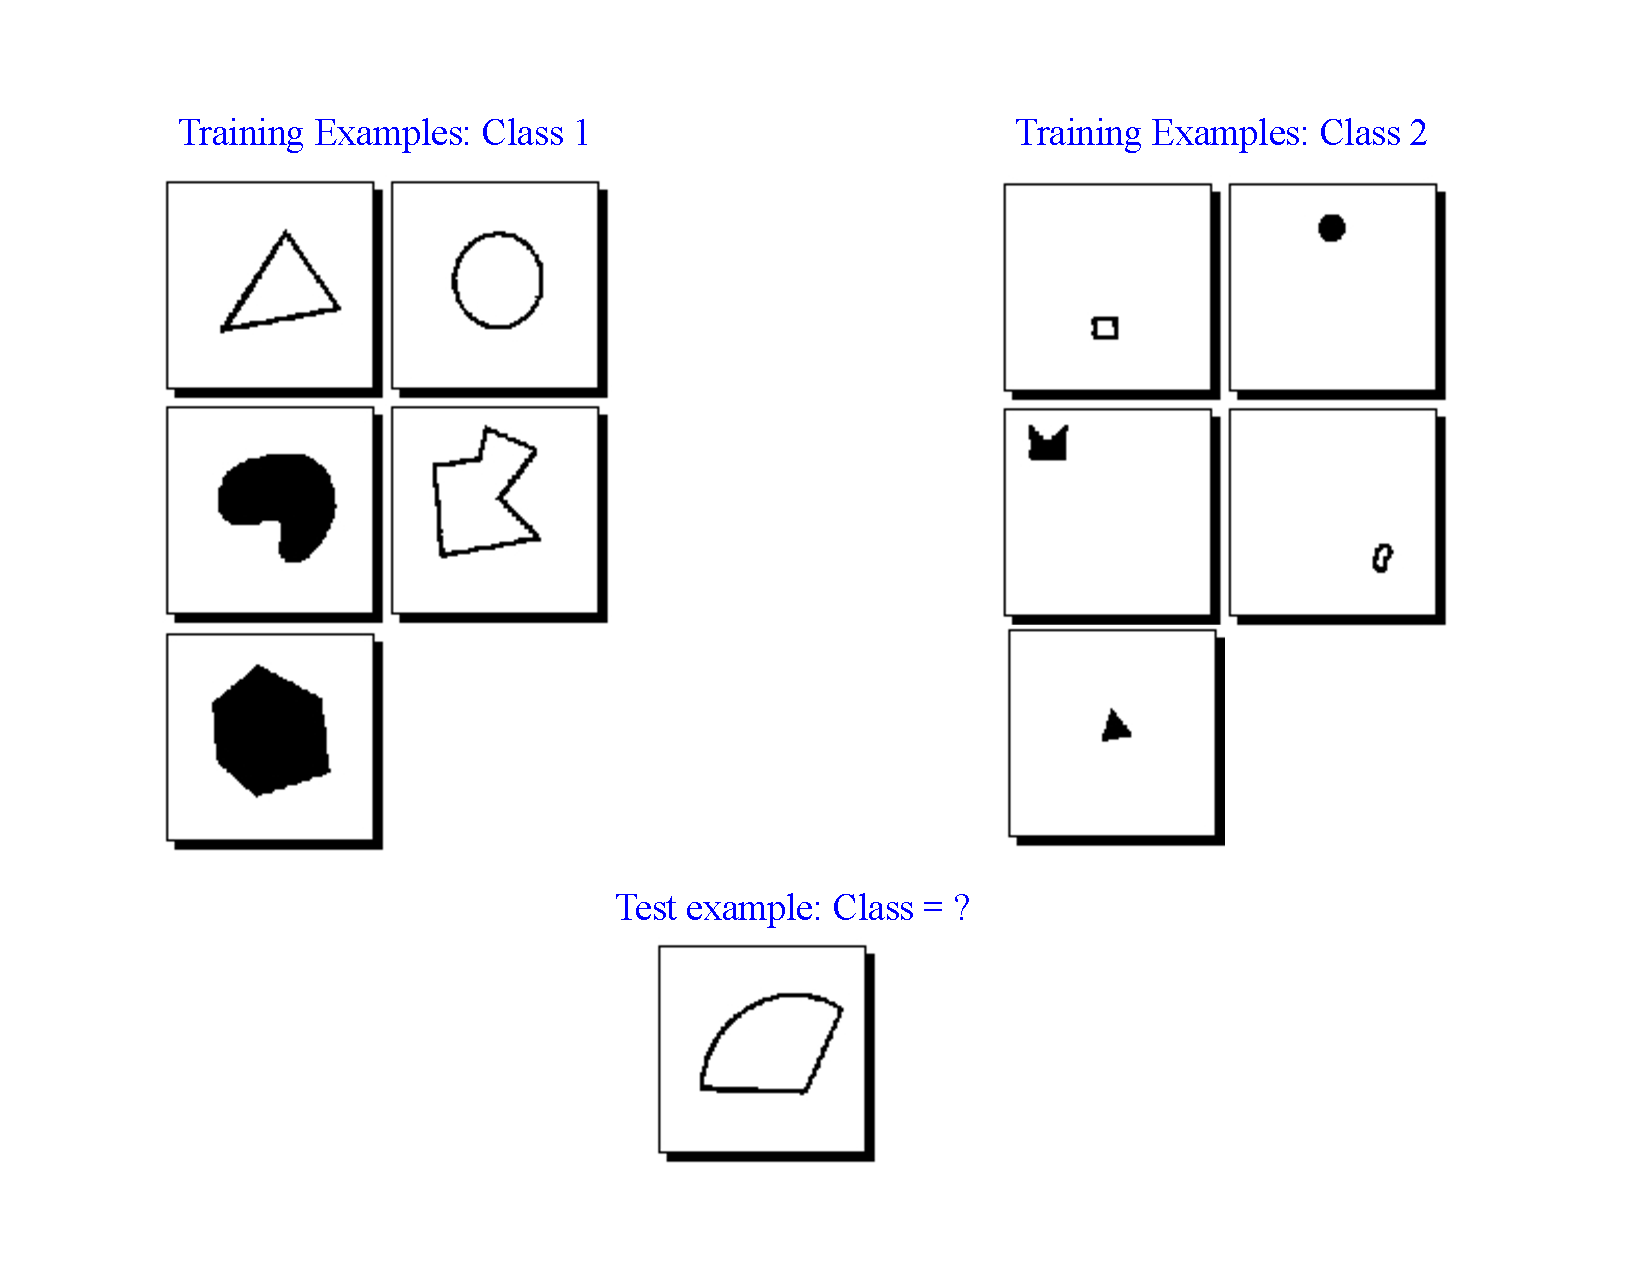
\includegraphics[scale=.4]{graphics/ML1}};  
 \end{tikzpicture}


\begin{textblock}{1}(.45,.85)
  \tiny{Dr. Melanie Mitchell, PSU CS545 "Machine Learning", Spring 2014}
\end{textblock}
\end{frame}

%---------------------------------------------
\begin{frame}{Machine Learning (ML)}

\begin{tikzpicture}[overlay]
  \node[anchor=south west] at (0,-4.5) {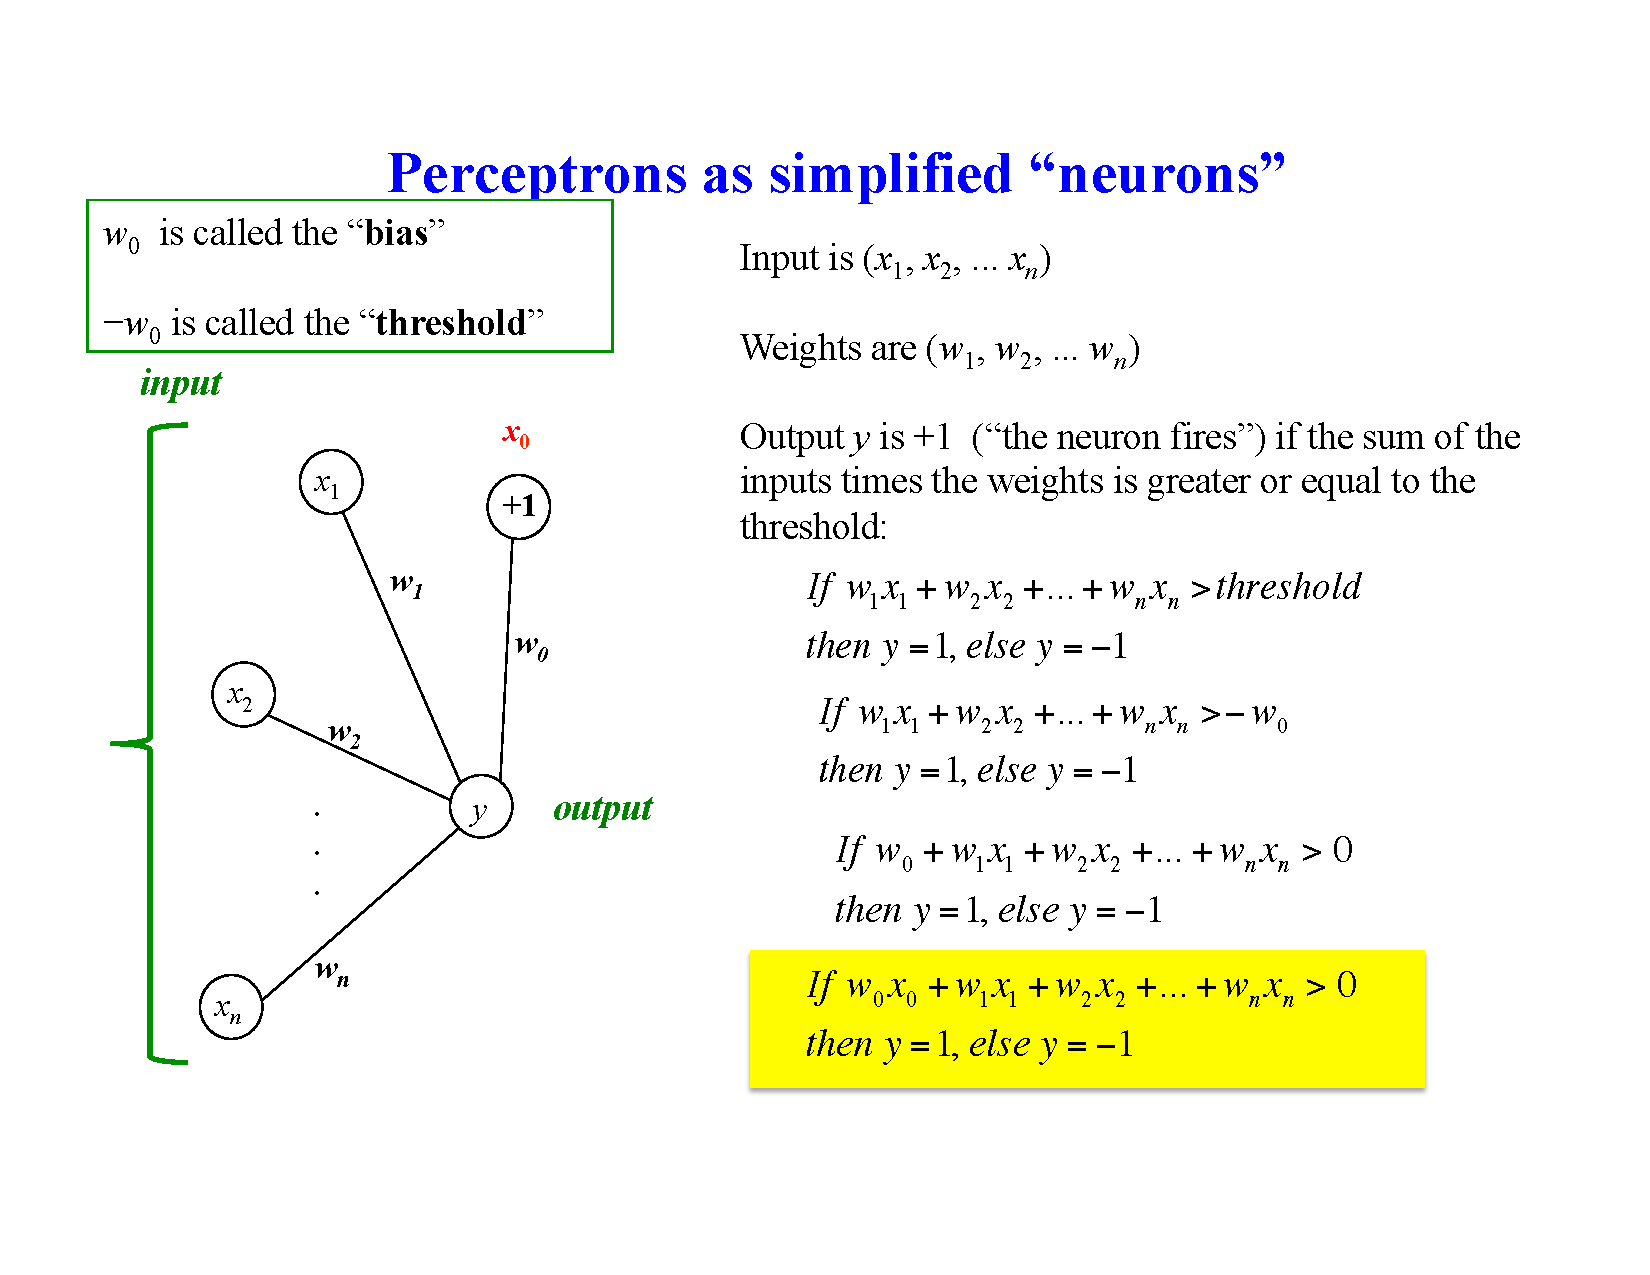
\includegraphics[scale=.4]{graphics/ML2}};  
 \end{tikzpicture}


\begin{textblock}{1}(.45,.85)
  \tiny{Dr. Melanie Mitchell, PSU CS545 "Machine Learning", Spring 2014}
\end{textblock}
\end{frame}


%----------------------------------
\section{A Few Definitions}
%-----------------------------------

%---------------------------------------------------------------
\begin{frame} {Acronyms in AI Translation}
 \begin{table}
\begin{tabular}{lll}
\textbf{LLM}  &   &    Large Language Model\\
\textbf{NMT}  &   &    Neural Machine Translation [Google] \\
\textbf{GPT } &   &    Generative Pre-trained Transformer	[OpenAI]\\
     &   & \\
\textbf{API}  &   &    Application Programming Interface\\
\textbf{SDK} &    &    Software Development Kit\\
\textbf{IDE } &   &    Integrated Development Environment\\
\textbf{MIME} &  & Multipurpose Internet Mail Extension; type of file format \\
\end{tabular}
\end{table}

\end{frame}

%----------------------------------
\section{Public AI Translators\\
(free with limitations)}
%---------------------------------------------------

%---------------------------------------------------
\begin{frame}{Google Translator - Simple Prose}

\begin{textblock}{1}(.05,.21)
  \normalsize {I love going to school! It's such a challenging environment.}
\end{textblock}\begin{textblock}{1}(.45,.85)
  \tiny{Dr. Melanie Mitchell, PSU CS545 "Machine Learning", Spring 2014}
\end{textblock}

\begin{tikzpicture}[overlay]
  \node[anchor=south west] at (0,-1) {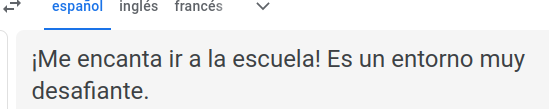
\includegraphics[scale=.5]{graphics/LoveSchool_Google.png}};  
 \end{tikzpicture}

\end{frame}

%--------------------------------------------------------------
\begin{frame} {Google Translator - Poetry}
\begin{textblock}{1}(.05,.21)
  \normalsize {\enquote{For what is it to die but to stand naked in the wind and to melt into the sun? And when the earth shall claim your limbs, then shall you truly dance.} (Kahlil Gibran, artist and poet)}
\end{textblock}

\begin{tikzpicture}[overlay]
  \node[anchor=south west] at (-1,-3) {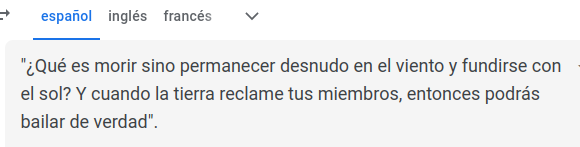
\includegraphics[scale=.6]{graphics/KahlilGilbran_Google.png}};  
 \end{tikzpicture}

\end{frame}

%---------------------------------------------------------------
\begin{frame} {Google Translator - Science Text}
\begin{textblock}{1}(.05,.21)
  \footnotesize {The Anthropocene is a proposed new geological epoch based on the observation that human impacts on essential planetary processes have become so profound that they have driven the Earth out of the Holocene epoch in which agriculture, sedentary communities, and eventually, socially and technologically complex human societies developed. The formalization of the Anthropocene as a new geological epoch is being considered by the stratigraphic community, but regardless of the outcome of that process, it is becoming apparent that Anthropocene conditions transgress Holocene conditions in several respects. The knowledge that human activity now rivals geological forces in influencing the trajectory of the Earth System has important implications for both Earth System science and societal decision making. [Steffen et. al. (2018) Trajectories of the Earth System in the Anthropocene, \textit{PNAS}]}
\end{textblock}

\end{frame}

%---------------------------------------------------------------
\begin{frame} {Google Translator - Science Text}
\begin{tikzpicture}[overlay]
  \node[anchor=south west] at (-1,-4.5) {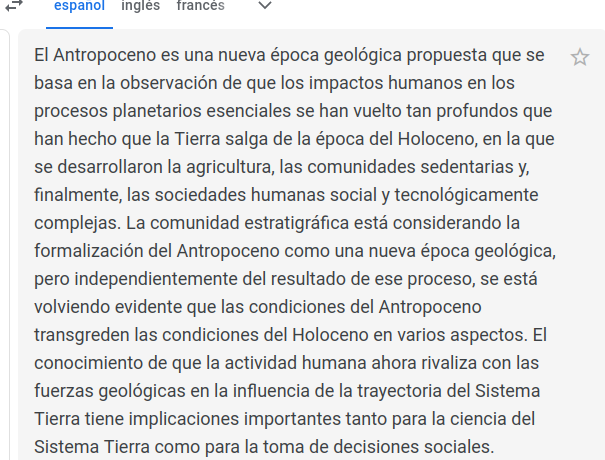
\includegraphics[scale=.5]{graphics/HotEarth_Google.png}};  
 \end{tikzpicture}
 
\end{frame}


%---------------------------------------------------------------
\begin{frame} {Google Translator - Legal Text}
\begin{textblock}{1}(.05,.21)
  \footnotesize {La Secretar\'ia del Trabajo y Previsi\'on Social deber\'a pronunciarse respecto de la solicitud de registro
dentro de los veinte d\'ias posteriores a la recepci\'on de la misma, de no hacerlo, los solicitantes podr\'an
requerirla para que dicte la resoluci\'on correspondiente, dentro de los tres d\'ias siguientes a la
presentaci\'on del requerimiento. Transcurrido dicho plazo sin que se notifique la resoluci\'on, se tendr\'a por
efectuado el registro para los efectos legales a que d\'e lugar. [Art\'iculo 15. LEY FEDERAL DEL TRABAJO, publicada 30-09-2024] }
\end{textblock}

\end{frame}

%---------------------------------------------------------------
\begin{frame} {Google Translator - Legal Text}
\begin{tikzpicture}[overlay]
  \node[anchor=south west] at (0.5,-1) {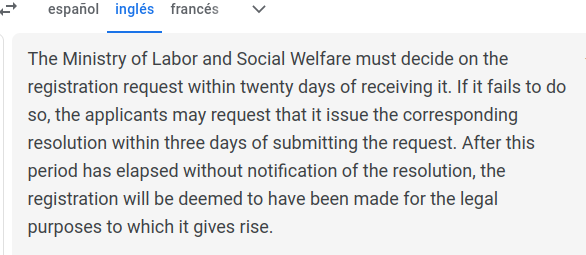
\includegraphics[scale=.5]{graphics/Law_Google.png}};  
 \end{tikzpicture}
 
 \begin{textblock}{1}(.05,.6)
  \footnotesize {The Ministry of Labor and Social Welfare (MLSW) must approve or reject the registration request within twenty days after its receipt in the offices of the MLSW. If the MLSW fails to do so, the applicants may formally require that the MLSW resolve the issue within three business days. If, after this second period has elapsed without notification of the status of the registration request, the registration request will be deemed approved for all applicable legal purposes. [\textit{Marron translation}]}
\end{textblock}
 
\end{frame}


%---------------------------------------------------------------
\begin{frame} {ChatGPT - Legal Text}

\begin{tikzpicture}[overlay]
  \node[anchor=south west] at (-1,-1) {
\includegraphics[scale=.4]{graphics/Law_GPT.png}};  
 \end{tikzpicture}

 
 \begin{textblock}{1}(.05,.6)
  \footnotesize {The Ministry of Labor and Social Welfare must issue a decision regarding the registration request within twenty days of receiving it. If it fails to do so, the applicants may formally request that the corresponding resolution be issued within three days following the submission of such a request. If this period elapses without notification of the resolution, the registration will be considered completed for all applicable legal purposes.}
\end{textblock}
 
\end{frame}



%-------------------------------------------------------------------
\section{Registered User AI Translators \\
(pay per limit)}
%-------------------------------------------------------------------

%-------------------------------------------------------------------
\begin{frame}{OpenAI API: GPT-4o}

\begin{textblock}{1}(.1,.2)
  \small {\textbf{GPT-4o:} A type of foundational LLM that can generate content in over 90 languages. Multiple types of rate limits apply. }
\end{textblock}


\begin{textblock}{1}(.1,.4)
  \footnotesize {\enquote{We're running GPT4 translations on english, german, french, spanish, italian, portugese, on a daily basis, and I can assure you it's the best available option hands down.}\\~\\
  \enquote{...the talk of the town with its very impressive language translation technology that's taking multilingual communication by storm. GPT-4 has the remarkable ability to analyze the context and meaning of words and sentences, which makes it able to make more accurate translations}\\~\\
  \enquote{...it generates text 2x faster and is 50\% cheaper. Additionally, GPT-4o has the best vision and performance across non-English languages of any of our models. \textbf{GPT-4o is available in the OpenAI API to paying customers.}}
}
\end{textblock}

\end{frame}


%-------------------------------------------------------------------
\begin{frame}{Access to GPT-4o API}

\begin{textblock}{1}(.1,.2)
  \footnotesize {Once you have applied for access, you must be reviewed and approved...

Once your application has been approved, you will receive an API key ...

Once you have gained access to the API, you will need to install the necessary SDK (using an IDE) ..... 

Once you have configured GPT-4 for your project, you need to initialize GPT-4 for translation....

And now you will be ready to start using the model for language translation.}
\end{textblock}

\begin{textblock}{1}(.5,.65)
  \normalsize{\textbf{Yikes!}}
\end{textblock}

\end{frame}

%-------------------------------------------------------------------
\begin{frame}{Google Cloud Translation API}

\begin{textblock}{1}(.1,.2)
  \footnotesize {This API uses a pre-trained, custom model or a translation specialized large language model (LLMs). You can choose from different models based on your needs, such as: 
\begin{itemize}
  \item \textbf{Neural Machine Translation (NMT):} For general text, like website content or news articles. Available in 194 languages! 
  \item \textbf{Translation Large Language Model (LLM):} For conversational text, like messages or social media posts 
  \item \textbf{AutoML Translation:} For highly specialized or technical content
\end{itemize}
}
\end{textblock}


\begin{textblock}{1}(.1,.65)
  \tiny{NB. Google Translate uses sequence-to-sequence models. These models also are used in voice-activated gadgets, and online chatbots.}
\end{textblock}


\end{frame}


%----------------------------------------------------------------
\section{AI vs. Human Translators: The Science}
%----------------------------------------------------------------

%----------------------------------------------------------------
\begin{frame}{Peer-Reviewed Science}

\begin{tikzpicture}[overlay]
  \node[anchor=south west] at (-0.6,0.5) {
\includegraphics[scale=.50]{graphics/Yan_1.png}};
 \end{tikzpicture}
 
 
 \begin{textblock}{1}(.1,.5)
  \small {To our knowledge, \textbf{this study is the first to evaluate LLMs against human translators} and analyze the systematic differences between their outputs, providing valuable insights into the current state of LLM-based translation and its potential limitations.}
\end{textblock}
 
\end{frame}



%----------------------------------------------------------------
\begin{frame}{Peer-Reviewed Science}

\begin{tikzpicture}[overlay]
  \node[anchor=south west] at (-0.6,2.5) {
\includegraphics[scale=.50]{graphics/Yan_2.png}};
 \end{tikzpicture}

\begin{textblock}{1}(.1,.4)
  \small {\textit{ABSTRACT} This study comprehensively evaluates the translation quality of Large Language Models (LLMs), specifically GPT-4, against human translators of varying expertise levels across multiple language pairs and domains... we find that \textbf{GPT-4 performs comparably to junior translators in terms of total errors made but lags behind medium and senior translators}....[we] find that \textbf{GPT-4 translator suffers from literal translations, but human translators sometimes overthink the background information}.}
\end{textblock}

\end{frame}


%----------------------------------------------------------------
\begin{frame}{Peer-Reviewed Science}

\begin{tikzpicture}[overlay]
  \node[anchor=south west] at (-0.6,2.5) {
\includegraphics[scale=.50]{graphics/Yan_2.png}};
 \end{tikzpicture}

\begin{textblock}{1}(.1,.4)
  \small {\textit{CONCLUSION} ... GPT-4 has made significant strides in approaching human-level translation quality...This suggests promising opportunities for collaboration and enhancement of translation workflows...we anticipate that \textbf{LLMs will become increasingly valuable tools in the translation industry, working alongside human translators to improve productivity, efficiency, and overall translation quality.}}
\end{textblock}

\end{frame}

%----------------------------------
\section{Natural Language Translation \\
in the 21\textsuperscript{st}  C.}
%-----------------------------------

%-------------------------------------------------------------------
\begin{frame}{Is AI a Threat to Human Language Translators?}

\large \textit{Perhaps, but unlikekly unless folks are unprepared. \\-\\
What is likely is that professional translators will increasingly be required to interface with LLMs through subscription-based APIs. This means adding machine language coding to your tool kit.}

\end{frame}

%-------------------------------------------------------------------
\begin{frame}{Using Google Cloud Translate API}

\large {Not trivial!!}

\end{frame}

%-------------------------------------------------------------------
\begin{frame}{My Adventures with Google Translate API:\\
google-cloud-sdk and google-cloud-translate}

\begin{tikzpicture}[overlay]
  \node[anchor=south west] at (-1,-3.3) {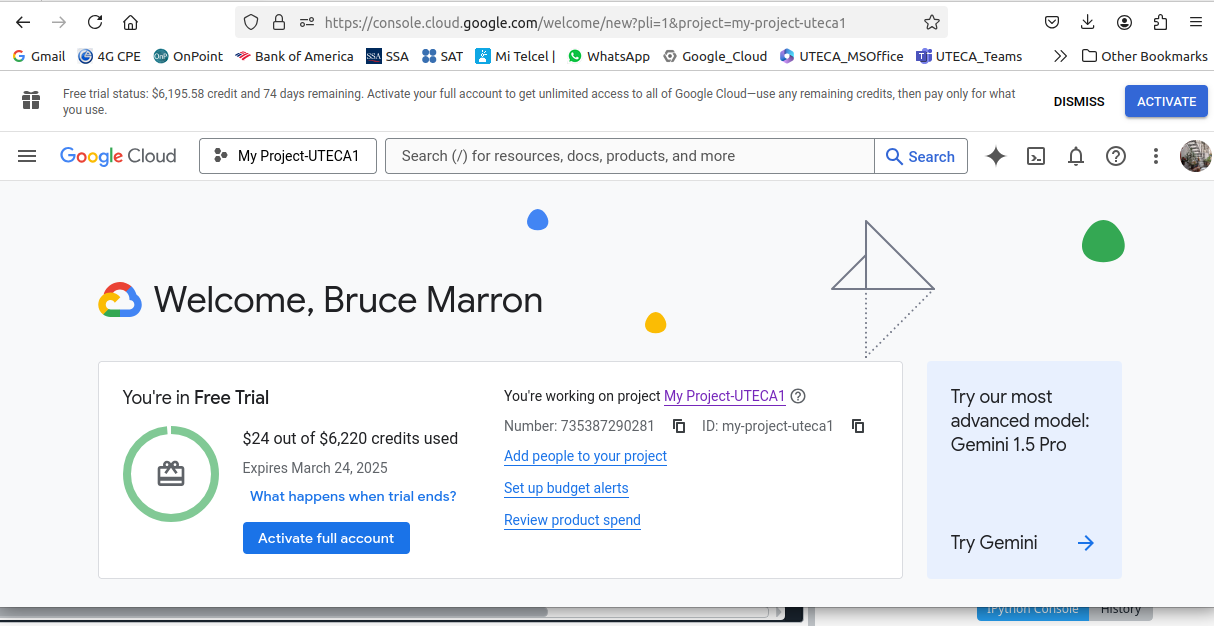
\includegraphics[scale=.28]{graphics/Google_1.png}};
 \end{tikzpicture}

\end{frame}

%-------------------------------------------------------------------
\begin{frame}{My Adventures with Google Translate API:\\
google-cloud-sdk and google-cloud-translate}

\begin{tikzpicture}[overlay]
  \node[anchor=south west] at (-1,-3.3) {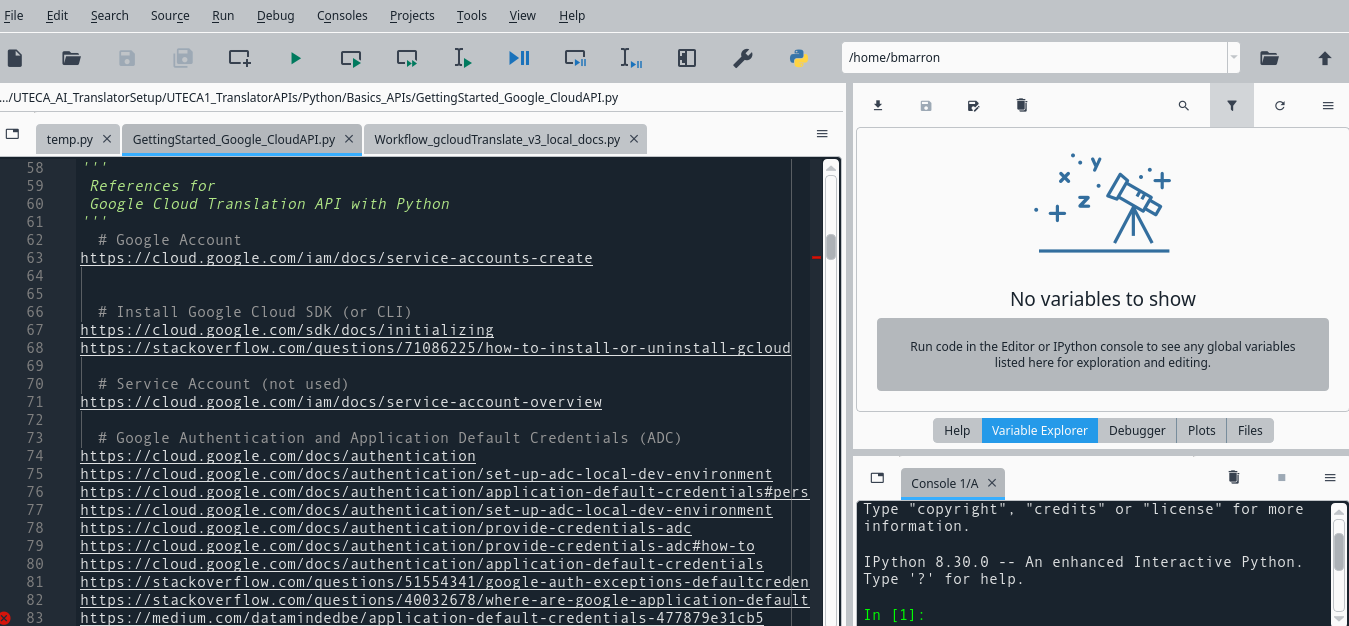
\includegraphics[scale=.28]{graphics/Python_1.png}};
 \end{tikzpicture}

\end{frame}

%-------------------------------------------------------------------
\begin{frame}{My Adventures with Google Translate API:\\
google-cloud-sdk and google-cloud-translate}

\begin{tikzpicture}[overlay]
  \node[anchor=south west] at (0,-4) {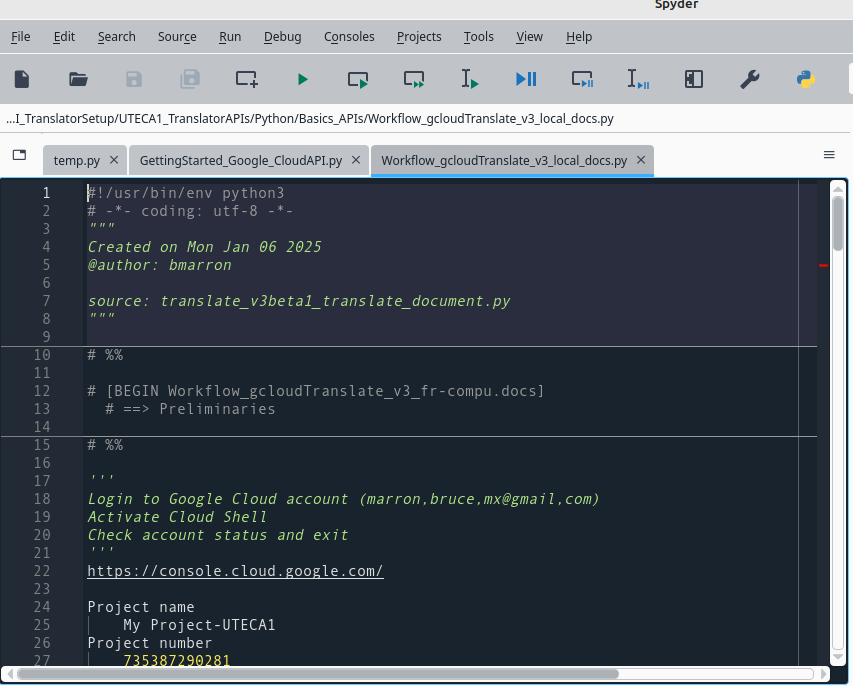
\includegraphics[scale=.31]{graphics/Python_2.png}};
 \end{tikzpicture}

\end{frame}

%-------------------------------------------------------------------
\begin{frame}{My Adventures with Google Translate API:\\
google-cloud-sdk and google-cloud-translate}

\begin{tikzpicture}[overlay]
  \node[anchor=south west] at (0,-4) {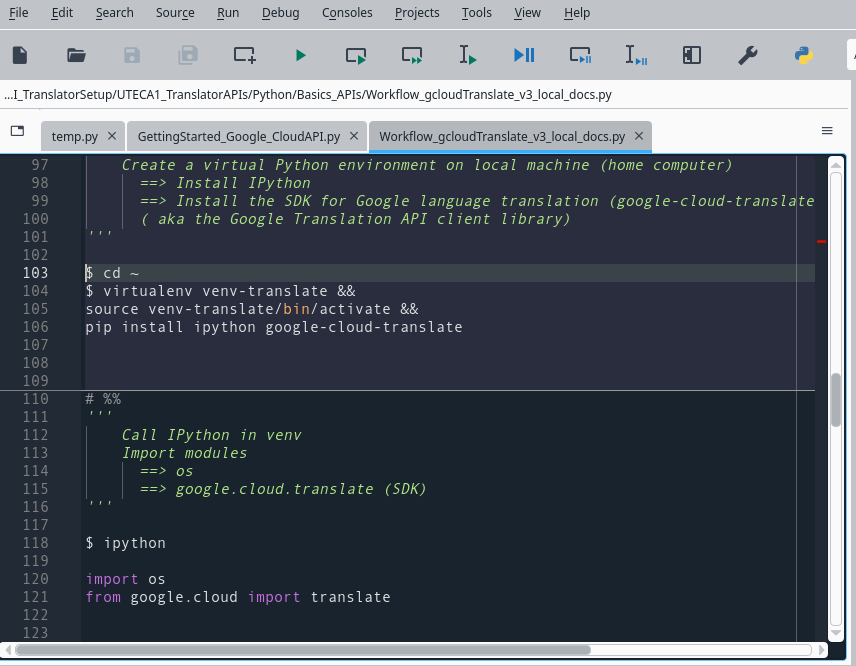
\includegraphics[scale=.31]{graphics/Python_3.png}};
 \end{tikzpicture}

\end{frame}

%-------------------------------------------------------------------
\begin{frame}{My Adventures with Google Translate API:\\
google-cloud-sdk and google-cloud-translate}

\begin{tikzpicture}[overlay]
  \node[anchor=south west] at (0,-4) {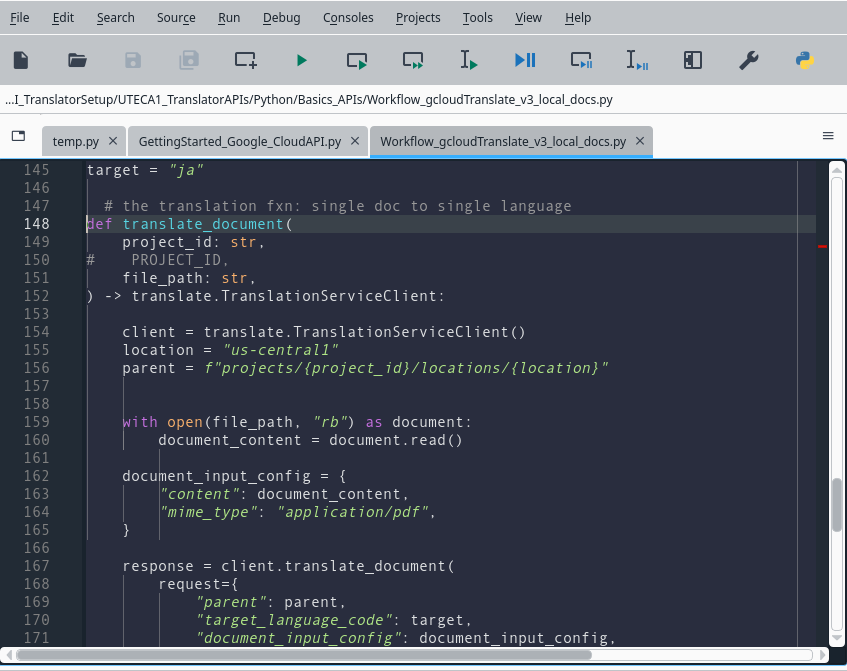
\includegraphics[scale=.31]{graphics/Python_4.png}};
 \end{tikzpicture}

\end{frame}

%-------------------------------------------------------------------
\begin{frame}{My Adventures with Google Translate API:\\
google-cloud-sdk and google-cloud-translate}

\begin{tikzpicture}[overlay]
  \node[anchor=south west] at (0,-4) {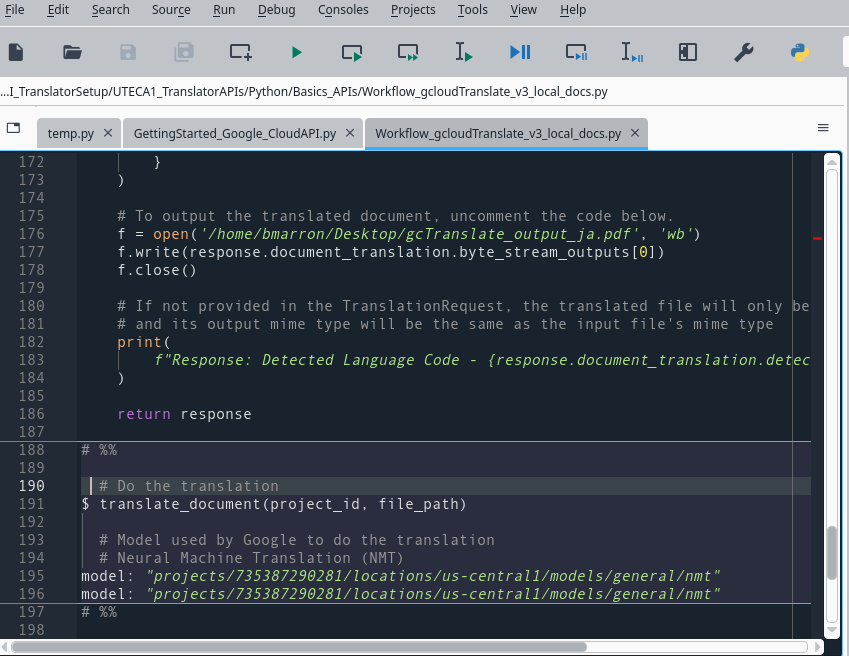
\includegraphics[scale=.31]{graphics/Python_5.png}};
 \end{tikzpicture}

\end{frame}

%-------------------------------------------------------------------
\begin{frame}{My Adventures with Google Translate API:\\
google-cloud-sdk and google-cloud-translate}

\begin{tikzpicture}[overlay]
  \node[anchor=south west] at (0,-4) {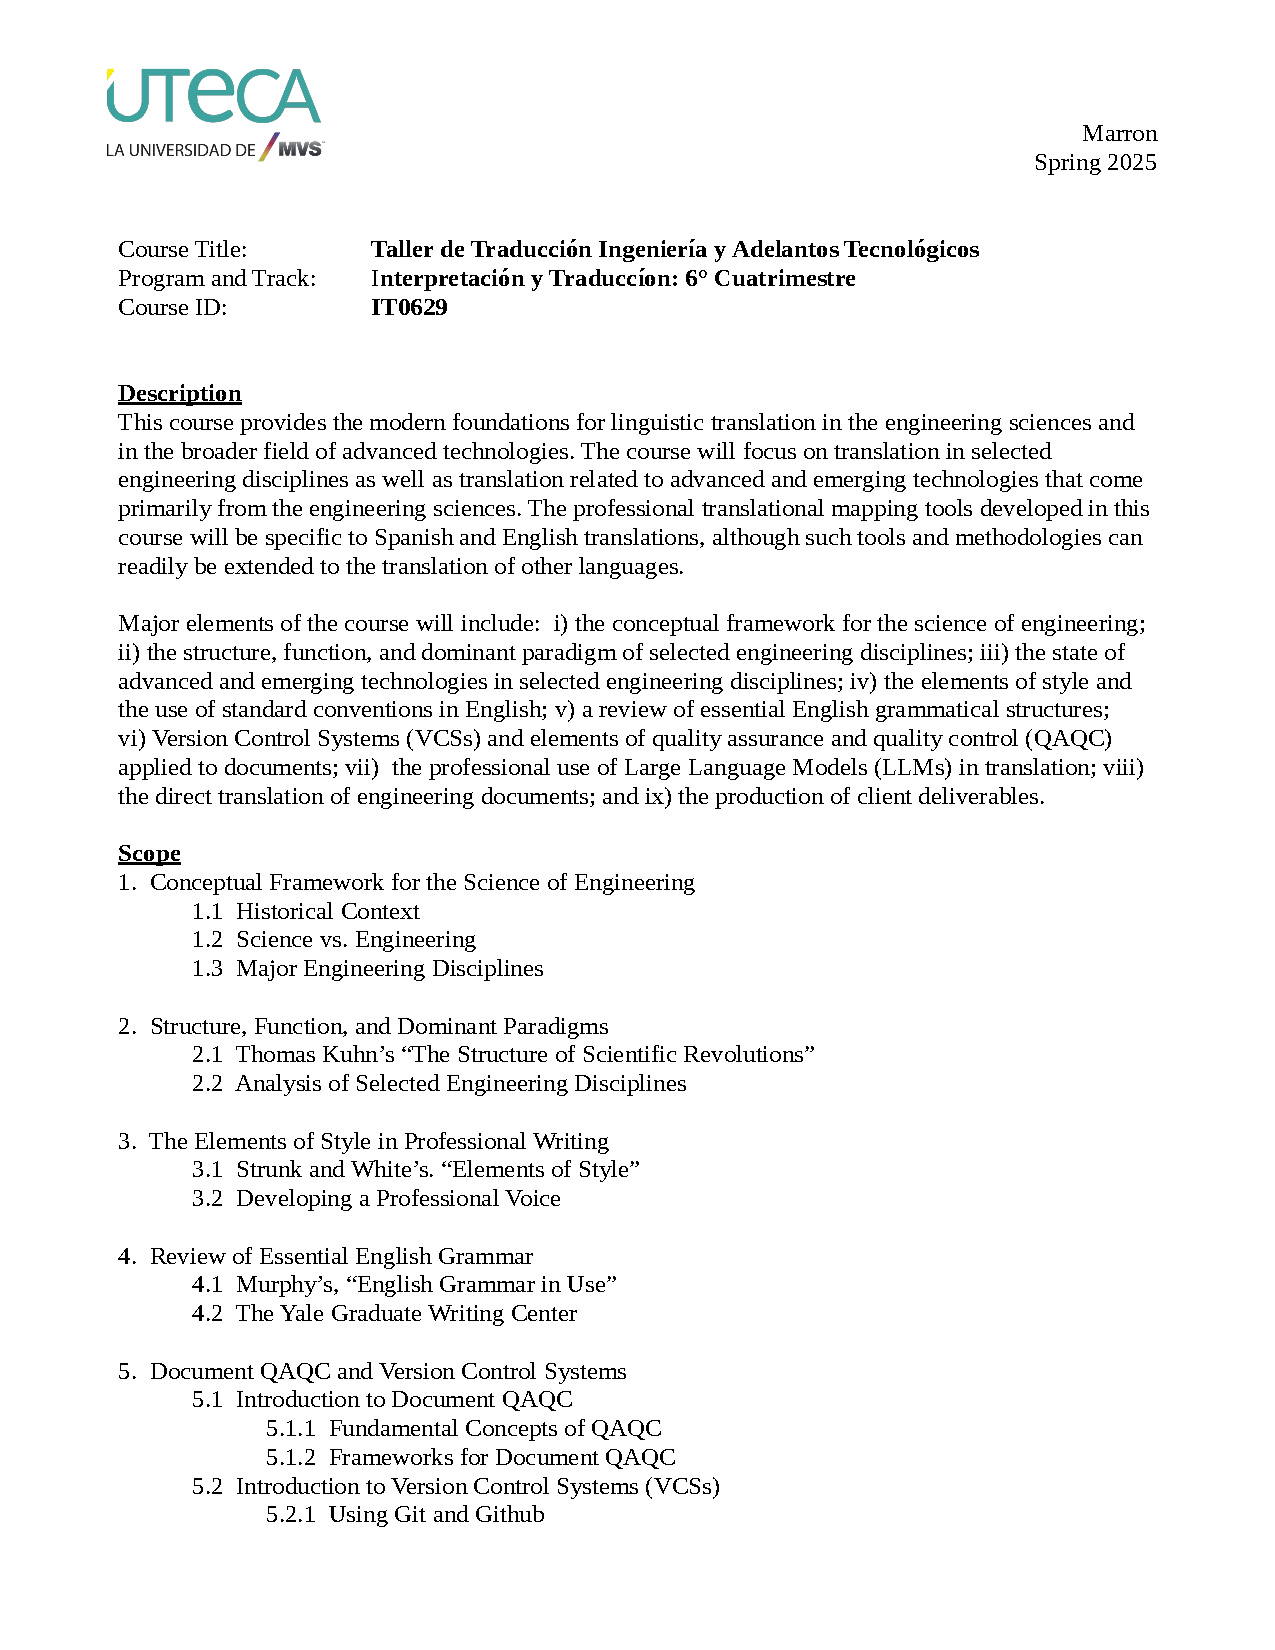
\includegraphics[scale=.27]{graphics/Original_Latex.pdf}};
\end{tikzpicture}

\begin{textblock}{1}(.65,.4)
  \footnotesize  {Course Description in .pdf format \\
Original language: English}
\end{textblock}

\end{frame}

%-------------------------------------------------------------------
\begin{frame}{My Adventures with Google Translate API:\\
google-cloud-sdk and google-cloud-translate}

\begin{tikzpicture}[overlay]
  \node[anchor=south west] at (0,-4) {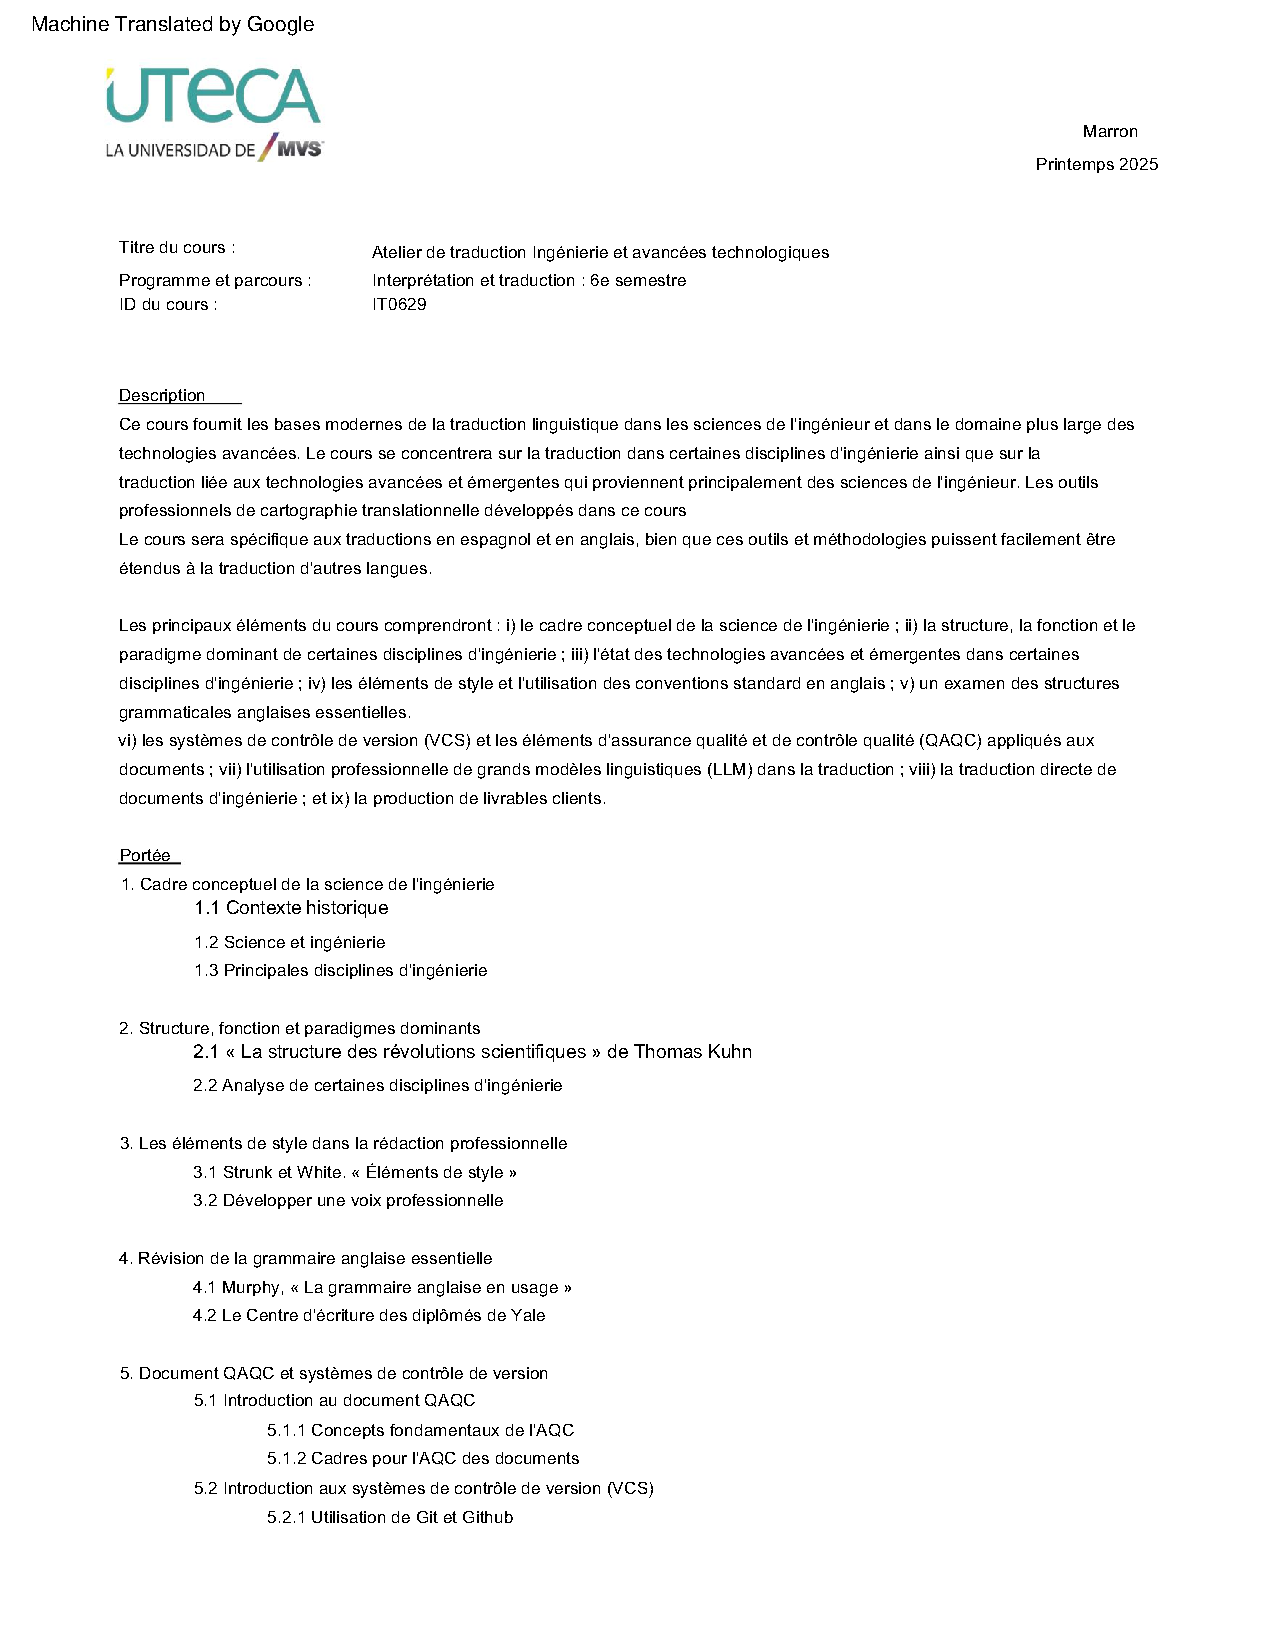
\includegraphics[scale=.27]{graphics/gcTranslate_output_fr_Latex.pdf}};
\end{tikzpicture}

\begin{textblock}{1}(.65,.4)
  \footnotesize  {Course Description in .pdf format \\
Translated language: French}
\end{textblock}

\end{frame}

%-------------------------------------------------------------------
\begin{frame}{My Adventures with Google Translate API:\\
google-cloud-sdk and google-cloud-translate}

\begin{tikzpicture}[overlay]
  \node[anchor=south west] at (0,-4) {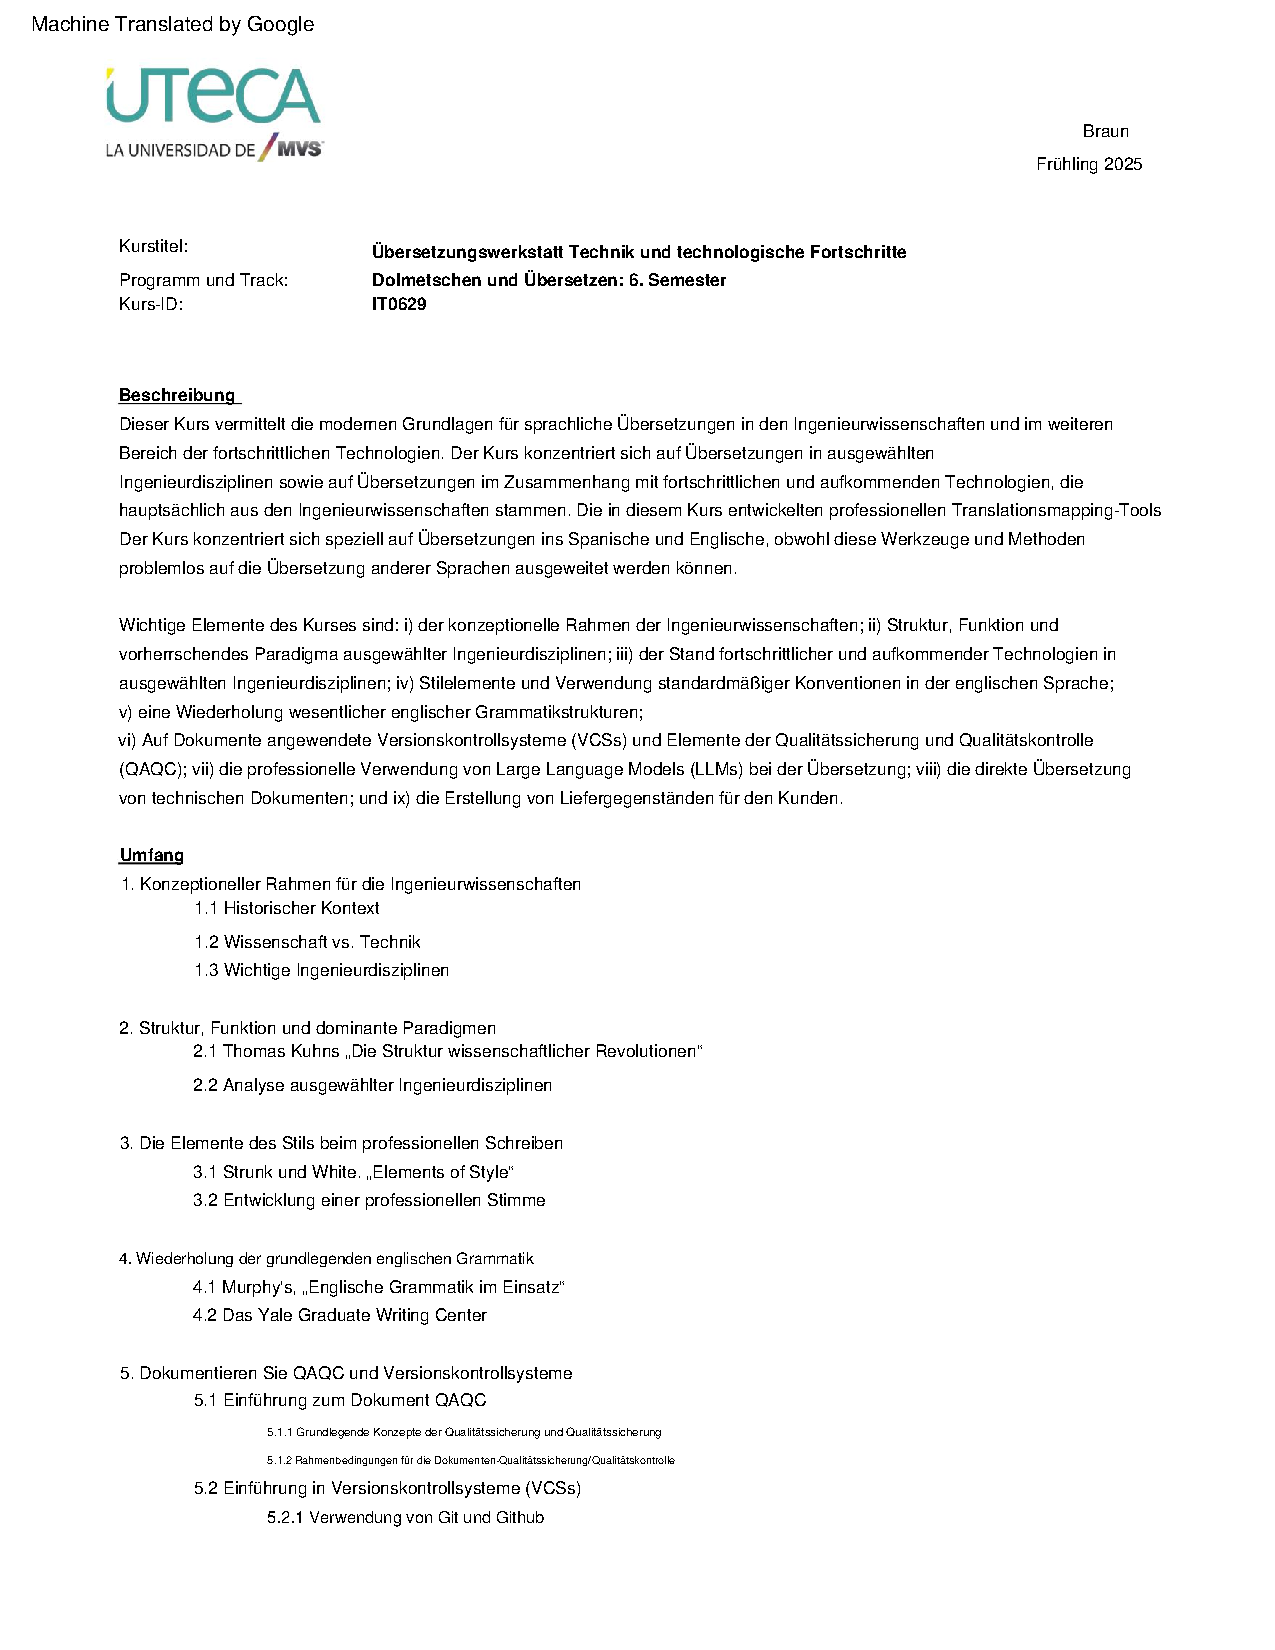
\includegraphics[scale=.27]{graphics/gcTranslate_output_de_Latex.pdf}};
\end{tikzpicture}

\begin{textblock}{1}(.65,.4)
  \footnotesize  {Course Description in .pdf format \\
Translated language: German}
\end{textblock}

\end{frame}


%-------------------------------------------------------------------
\begin{frame}{My Adventures with Google Translate API:\\
google-cloud-sdk and google-cloud-translate}

\begin{tikzpicture}[overlay]
  \node[anchor=south west] at (0,-4) {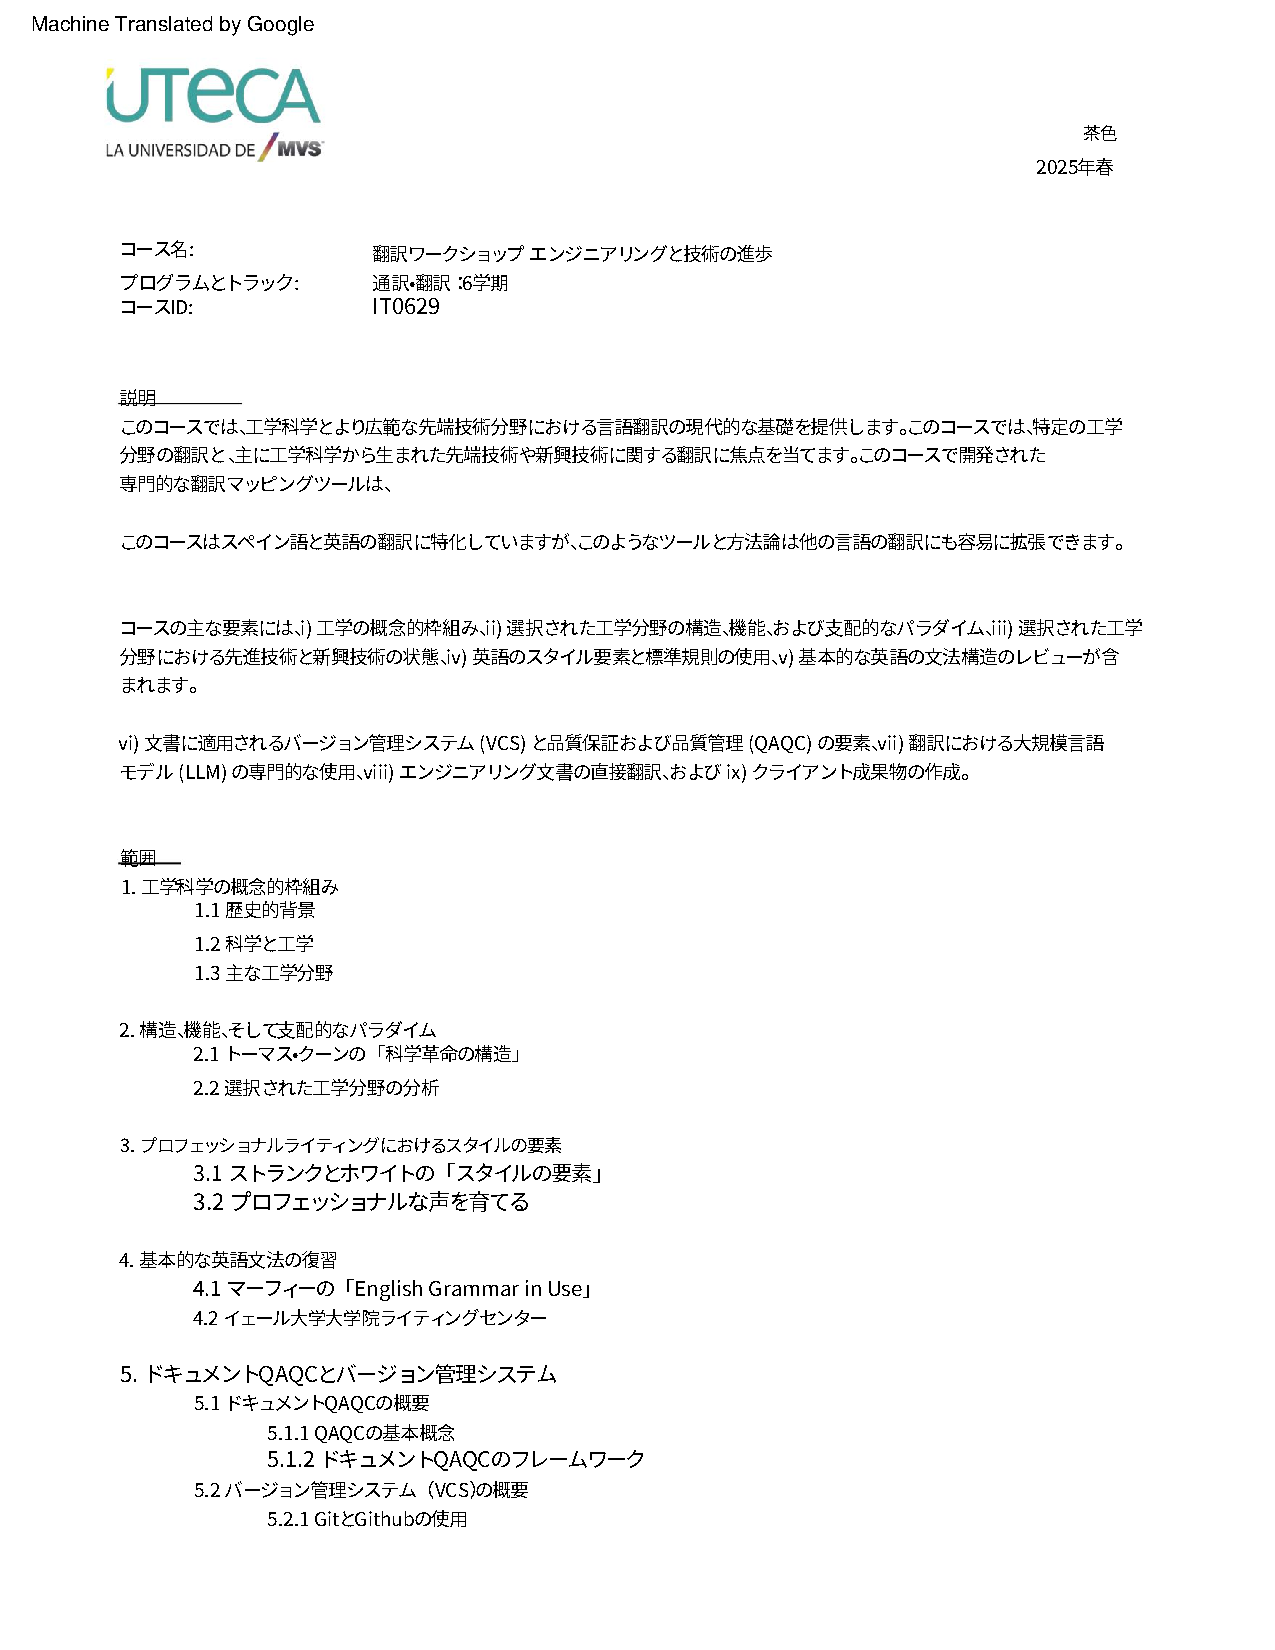
\includegraphics[scale=.27]{graphics/gcTranslate_output_ja_Latex.pdf}};
\end{tikzpicture}

\begin{textblock}{1}(.65,.4)
  \footnotesize  {Course Description in .pdf format \\
Translated language: Japanese}
\end{textblock}

\end{frame}

%-------------------------------------------------------------------
\begin{frame}{My Adventures with Google Translate API:\\
google-cloud-sdk and google-cloud-translate}

\begin{textblock}{1}(.5,.3)
\textbf{Translation Stats}
\end {textblock}


\begin{textblock}{1}(.05,0.4)
\begin{description}
  \item [MIME type] application/pdf 
  \item [No. Pages] 3
  \item [Processing Time] 7 sec
  \item [Cost per translated doc] 8 MXN
\end{description}

\end {textblock}

\end{frame}


%----------------------------------
\section{Recommendations}
%-----------------------------------

%----------------------------------------------------------------
\begin{frame}{The 21\textsuperscript{st}  C. Professional Translator}

\begin{tikzpicture}[overlay]
  \node[anchor=south west] at (-0.1,2.5) {
\includegraphics[scale=.15]{graphics/Anaconda.png}};
  \node[anchor=south west] at (5,2.5) {
\includegraphics[scale=.05]{graphics/Spyder.png}};
\end{tikzpicture}

\begin{textblock}{1}(.05,.3)
\begin{description}
  \item [Learn Python] The world's Python resources are huge! Anaconda is an open ecosystem for
sourcing, building, and deploying data science and AI initiatives. Spyder is a solid IDE.
  \item [Apply for a Google Cloud Account] Trial account gives you 6000 MXN and 90 days
  \item [Learn Google Cloud Client Libraries] google-cloud-sdk and google-cloud-translate to start
  \item [Begin translating with Google's API for Python!]
\end{description}

\end{textblock}

\end{frame}

%----------------------------------
\section{The Future}
%-----------------------------------

%----------------------------------------------------------------
\begin{frame}{Smartling}

\begin{tikzpicture}[overlay]
  \node[anchor=south west] at (0.0,-0.1) {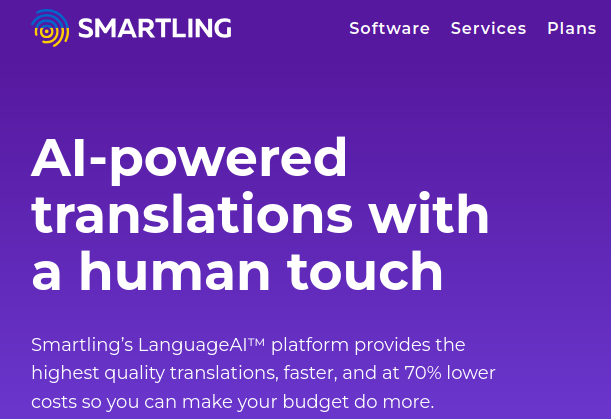
\includegraphics[scale=.2]{graphics/Smartling1.png}};
 \end{tikzpicture}

\begin{tikzpicture}[overlay]
  \node[anchor=south west] at (-0.05,-1.8) {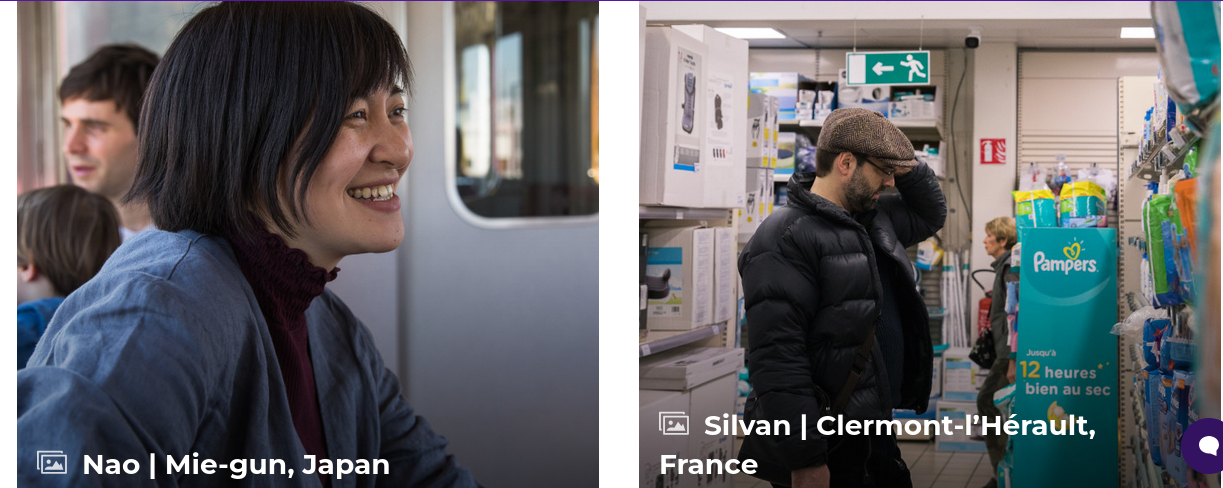
\includegraphics[scale=.15]{graphics/Smartling4.png}};
 \end{tikzpicture}
 
 \begin{tikzpicture}[overlay]
  \node[anchor=south west] at (-0.05,-3.8) {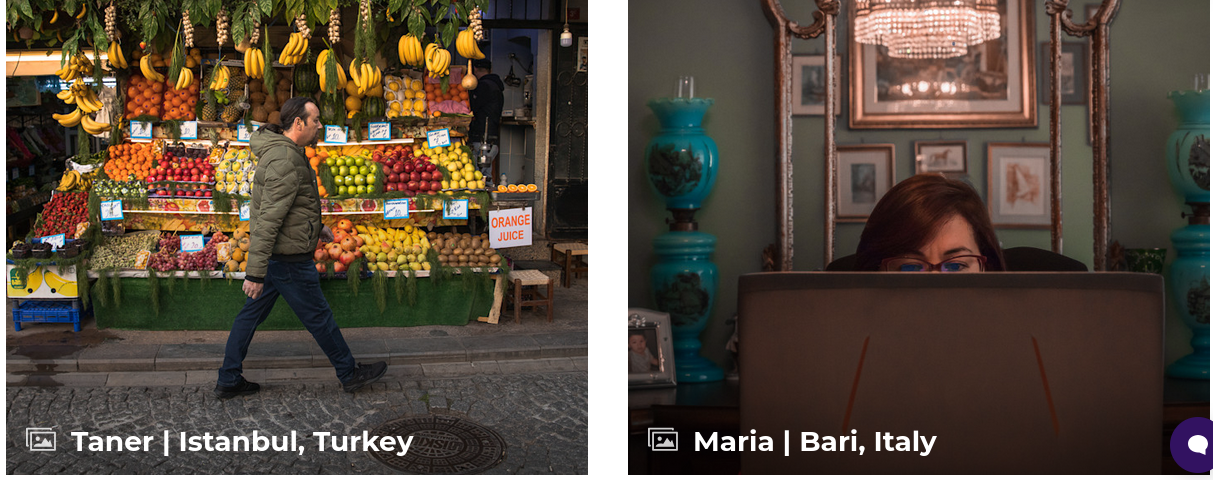
\includegraphics[scale=.15]{graphics/Smartling3.png}};
 \end{tikzpicture}

\end{frame}


%----------------------------------
\section{Thank you!}
%-----------------------------------



%######################################
% END DOC
%######################################
\end{document}
